\section{Khung mô hình kinh doanh (Business Model Canvas)}

Để tối ưu hóa quy trình vận hành và tạo ra giá trị bền vững cho cả người chơi và chủ sân, hệ thống áp dụng khung mô hình kinh doanh (Business Model Canvas) với các thành phần chính như sau:

\begin{figure}[H]
    \centering
    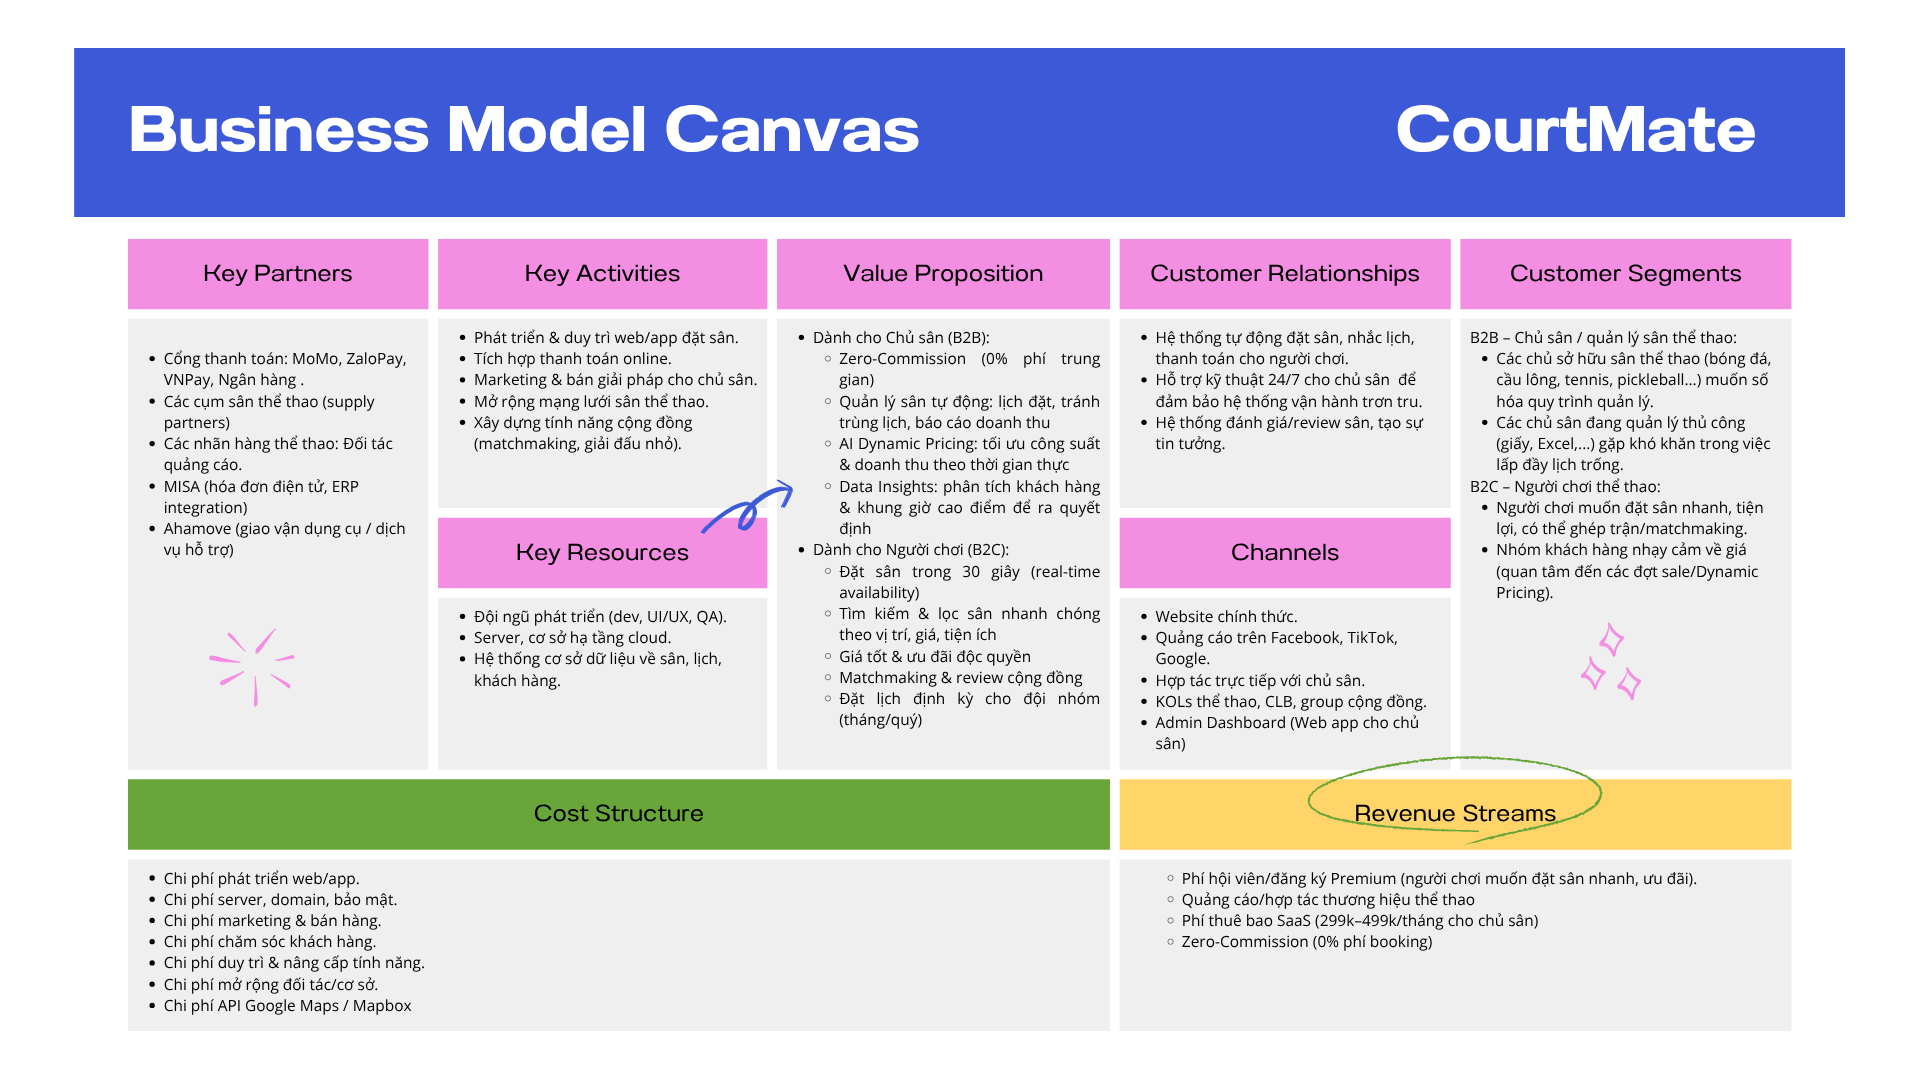
\includegraphics[width=1\textwidth]{Images/BMC.png}
    \caption{Khung mô hình kinh doanh (Business Model Canvas) của hệ thống CourtMate}
    \label{fig:bmc}
\end{figure}


\subsection{Chi tiết các thành phần trong mô hình}

\begin{enumerate}
    \item \textbf{Phân khúc khách hàng (Customer Segments):}
    \begin{itemize}
        \item \textbf{B2B (Chủ sân/Người quản lý):} Các chủ sở hữu cụm sân thể thao cần công cụ quản lý chuyên nghiệp, tự động hóa và báo cáo tài chính chính xác.
        \item \textbf{B2C (Người chơi thể thao):} Cá nhân hoặc nhóm người chơi cần tìm kiếm và đặt sân nhanh chóng, minh bạch về giá cả và tiện ích.
    \end{itemize}

    \item \textbf{Giải pháp giá trị (Value Propositions):}
    \begin{itemize}
        \item \textbf{Cho chủ sân:} Giảm thiểu sai sót thủ công, tối ưu hóa công suất khai thác sân (đặc biệt là giờ thấp điểm), quản lý tài chính tích hợp hóa đơn điện tử.
        \item \textbf{Cho người chơi:} Trải nghiệm đặt sân trong 30 giây; hiển thị trạng thái sân thời gian thực; tích hợp thanh toán linh hoạt; hệ thống Matchmaking tự động ghép trận và tính năng Recurring Booking cho phép đặt lịch cố định dài hạn.
    \end{itemize}

    \item \textbf{Các kênh truyền thông và phân phối (Channels):}
    \begin{itemize}
        \item Ứng dụng Web/Mobile cho người chơi.
        \item Bảng điều khiển (Admin Panel) chuyên dụng cho chủ sân.
        \item Mạng xã hội và các diễn đàn cộng đồng thể thao.
    \end{itemize}

    \item \textbf{Quan hệ khách hàng (Customer Relationships):}
    \begin{itemize}
        \item Hỗ trợ kỹ thuật 24/7 cho các chủ sân SaaS.
        \item Hệ thống đánh giá và phản hồi đa chiều giữa người chơi và chủ sân.
    \end{itemize}

    \item \textbf{Dòng doanh thu (Revenue Streams):}
    \begin{itemize}
        \item \textbf{B2B (SaaS):} Phí thuê bao hàng tháng từ chủ sân với cam kết 0\% hoa hồng, giúp họ tối ưu hóa lợi nhuận biên.
        \item \textbf{B2C (Premium):} Gói hội viên cao cấp dành cho người chơi để nhận ưu đãi, quét mã giảm giá và miễn phí phí ghép trận.
        \item \textbf{B2B2C (Ads):} Doanh thu quảng cáo từ các thực thể thương mại và nhãn hàng thể thao tài trợ.
    \end{itemize}

    \item \textbf{Các hoạt động chính (Key Activities):}
    \begin{itemize}
        \item Phát triển và bảo trì nền tảng kỹ thuật.
        \item Kết nối và mở rộng mạng lưới các đối tác cụm sân.
        \item Tiếp thị và chăm sóc khách hàng.
    \end{itemize}

    \item \textbf{Các nguồn lực chính (Key Resources):}
    \begin{itemize}
        \item Đội ngũ kỹ sư phát triển phần mềm.
        \item Hạ tầng máy chủ Cloud và cơ sở dữ liệu.
        \item Dữ liệu về bản đồ và vị trí các cụm sân.
    \end{itemize}

    \item \textbf{Các đối tác chính (Key Partners):}
    \begin{itemize}
        \item \textbf{Thanh toán:} MoMo, ZaloPay xử lý giao dịch tức thời và bảo mật.
        \item \textbf{Công nghệ \& Vận hành:} MISA meInvoice (hóa đơn điện tử); Ahamove (giao vận dụng cụ/nhu yếu phẩm).
        \item \textbf{Thương mại:} Các nhãn hàng thể thao tài trợ và quảng cáo trên nền tảng.
    \end{itemize}

    \item \textbf{Cơ cấu chi phí (Cost Structure):}
    \begin{itemize}
        \item Chi phí vận hành hạ tầng Cloud (AWS/Azure).
        \item Phí sử dụng API Google Maps.
        \item Chi phí nhân sự và Marketing.
    \end{itemize}
\end{enumerate}
